\subsection{Ziel} \label{sec:goal}

Dieses Kapitel umfasst die Zielbeschreibung und ist damit als erstes Kapitel besonders wichtig um dem Leser verständlich zu machen was dieses Dokument umfassen soll.
Insgesamt ist das hier nur ein Fülltext, welcher etwas Inhalt darstellen soll und nur als Beispiel dient.

Beispielweise wie man einen neuen Absatz beginnt oder eine Bild einfügt.

\begin{figure}[htb]
    \centering
    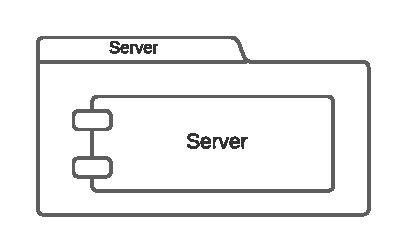
\includegraphics[scale=.65,center]{medien/diagrams/server}
    \caption{Bild mit einem Diagram}
    \ownsource
    \label{fig:server-diagram}
\end{figure}

\begin{figure}
\centering
\begin{subfigure}{.5\textwidth}
  \centering
  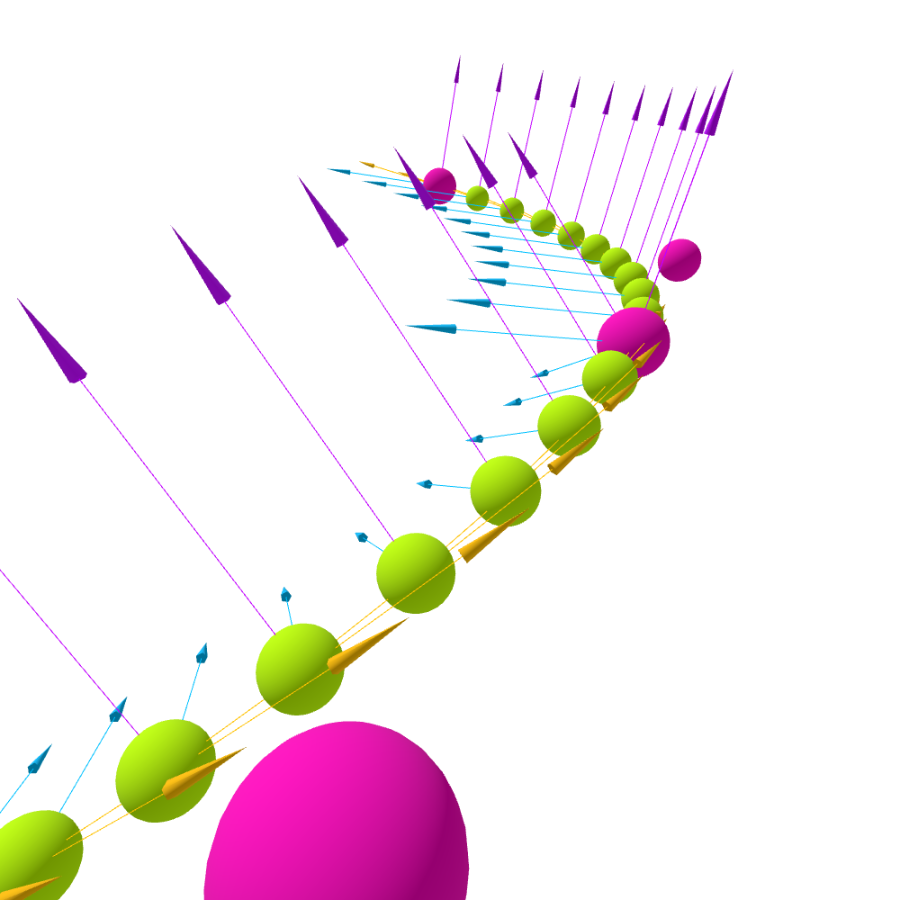
\includegraphics[width=.4\linewidth]{medien/render-shots/front}
  \caption{A subfigure}
  \label{fig:sub1}
\end{subfigure}%
\begin{subfigure}{.5\textwidth}
  \centering
  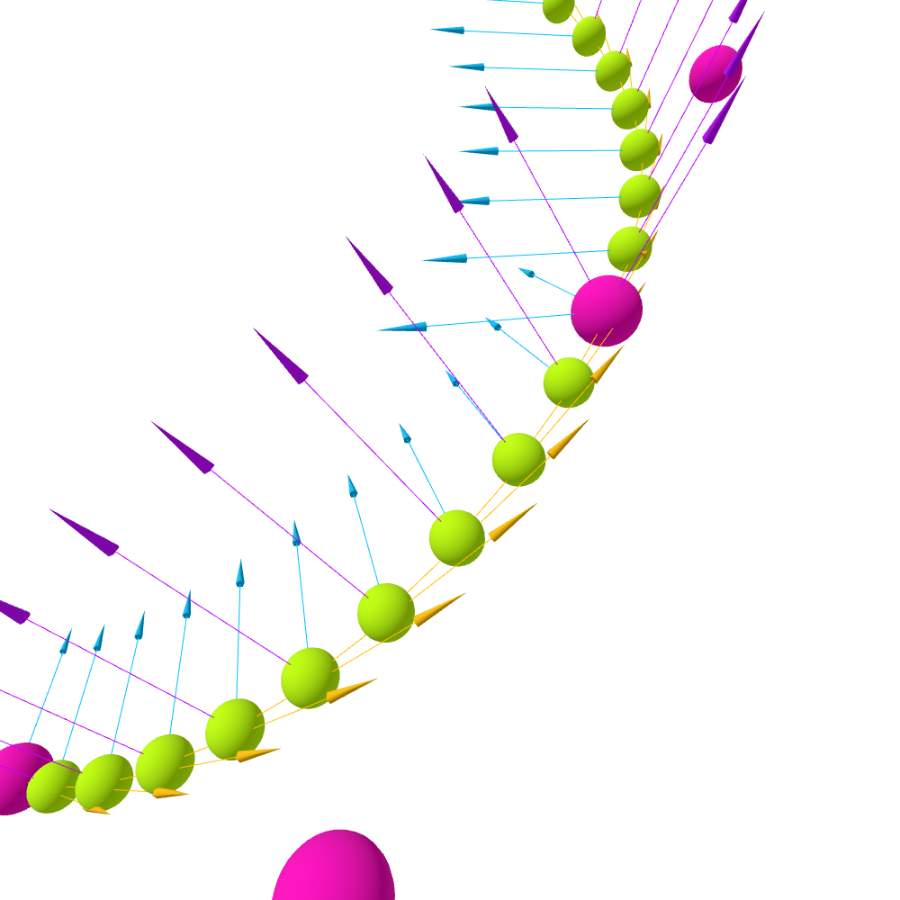
\includegraphics[width=.4\linewidth]{medien/render-shots/top}
  \caption{A subfigure}
  \label{fig:sub2}
\end{subfigure}
\caption{A figure with two subfigures and a caption}
\label{fig:test}
\end{figure}

% Die \FloatBarrier erlaubt Bilder zu zwingen spätestens an dieser Stelle zu erscheinen

Oder wie man Abschnitte referenziert \refsec{sec:goal} oder das eben eingefügte Bild \refimg{fig:server-diagram}.

Die plant uml Diagramme werden im Build step mitgebaut und dann ebenfalls unter Medien hinterlegt.
Deshalb können sie ebenfalls so referenziert werden.

\begin{figure}[htb]
    \centering
    \includegraphics[scale=.65,center]{medien/plant/minimal-client-server}
    \caption{Bild mit einem Client Server Diagram}
    \ownsource
    \label{fig:minimal-client-server-diagram}
\end{figure}

\FloatBarrier

Wenn source code rendering eingeschaltet ist kann dieser dann folgendermaßen eingebunden werden.

\begin{listing}[htb]
   \begin{minted}[linenos,fontsize=\normalsize]{TypeScript}
for(let i: number = 0; i < 12; i++)
   console.log("This is a test", i);
   \end{minted}
   \caption{Minimales TypeScript Beispiel}
   \ownsource
   \label{lis:ts-example}
\end{listing}

Natürlich kann auch dieser referenziert werden \reflis{lis:ts-example}.

Einträge aus dem Bibliography Kapitel lassen sich via\autocite{tensorflowTut2022} referenzieren und werden dann in dem entsprechenden Kapitel angezeigt.
Darüber hinaus lassen sich durch\footnote{\url{https://www.google.de}} Fußnoten Verweise und Referenzen erzeugen.

Tabellen sind weitere Elemente welche eingesetzt werden können.

\begin{table}[htb]
    \footnotesize{
        \makebox[\textwidth][c]{
            \begin{tabular}{ |r|r|r|r|r|r|r|r|r|  }
                \hline
                \multirow[b]{3}{4em}{Einheiten} & \multicolumn{4}{c|}{Client} & \multicolumn{4}{c|}{Server} \\
                \cline{2-9}
                & \multicolumn{2}{c|}{Rendering} & \multicolumn{2}{c|}{Deserializing} & \multicolumn{2}{c|}{Serializing} & \multicolumn{2}{c|}{Step} \\
                \cline{2-9}
                & Time    & Rate       & Time    & Rate       & Time    & Rate       & Time   & Rate        \\
                \hline
                256    & 0,63ms  & 1.585,20Hz & 0,21ms  & 4.660,19Hz & 0,47ms  & 2.150,11Hz & 0,03ms & 29.408,88Hz \\
                512    & 0,75ms  & 1.325,23Hz & 0,39ms  & 2.561,37Hz & 0,82ms  & 1.215,89Hz & 0,04ms & 25.365,15Hz \\
                1.024  & 0,99ms  & 1.010,10Hz & 0,79ms  & 1.273,21Hz & 1,19ms  & 840,96Hz   & 0,05ms & 20.244,45Hz \\
                2.048  & 1,38ms  & 726,39Hz   & 1,47ms  & 678,16Hz   & 2,47ms  & 404,14Hz   & 0,21ms & 4.671,12Hz  \\
                4.096  & 2,86ms  & 349,96Hz   & 3,43ms  & 291,16Hz   & 4,56ms  & 219,22Hz   & 0,48ms & 2.103,71Hz  \\
                8.192  & 7,97ms  & 125,54Hz   & 9,46ms  & 105,68Hz   & 10,19ms & 98,16Hz    & 0,70ms & 1.435,29Hz  \\
                16.384 & 14,27ms & 70,09Hz    & 20,51ms & 48,76Hz    & 27,20ms & 36,76Hz    & 0,73ms & 1.377,13Hz  \\
                32.768 & 31,60ms & 31,65Hz    & 41,25ms & 24,24Hz    & 40,77ms & 24,53Hz    & 1,31ms & 766,04Hz    \\
                \hline
            \end{tabular}
        }
    }
    \caption{Tabelle mit Daten}
    \ownsource
    \label{tbl:table-with-data}
\end{table}

\textit{Time} und \textbf{Rate} sind Möglichkeiten die Texte noch anderweitig hervorzuheben.
Bei jeder Änderung kann, wie in der README beschrieben, das Dokument neu gebaut werden.
Die erste Kompilation dauert einen kleinen Moment, die Nachfolgenden sind bedeutend schneller.
